\documentclass[a4paper,12pt]{article}

% PCIM Mandatory Margin Setup
\usepackage[top=2.2cm, bottom=3.0cm, left=1.7cm, right=1.7cm]{geometry}
\usepackage{graphicx}
\usepackage{amsmath}
\usepackage{caption}
\captionsetup[figure]{name=Fig.}
\usepackage{titlesec}
\usepackage{mathptmx}
\usepackage{algorithm}
\usepackage{algpseudocode}
\usepackage{indentfirst}
\setlength{\parindent}{2em}

% Heading formatting to match PCIM style
\titleformat{\section}{\normalfont\large\bfseries}{\thesection}{1em}{}
\titleformat{\subsection}{\normalfont\normalsize\bfseries}{\thesubsection}{1em}{}

\begin{document}

\begin{center}
    % Title strictly under 100 characters incl. spaces, Initial Letters Capitalized
    {\Large \bfseries A Robust PPO-based Control Scheme for 1 MHz DC-DC Converters with Multi-Domain Disturbance} \\[1em]
\end{center}

\noindent \textbf{Topic number and topic name:} 17.1 AI based control of DC-DC And AC-AC Converters\\
\textbf{Preferred presentation form:} Oral presentation \\[1em]
\vspace{-10pt}  % 根据需要调整数值（负值减小间距）
\noindent {\large \textbf{Abstract}}\\

A proximal policy optimization (PPO) strategy is proposed for 1 MHz DC-DC converters to achieve high-precision regulation and multi-condition robustness. Deployed on a fully parallelized FPGA inference engine, the model-free agent achieves sub-microsecond execution with sub-watt digital overhead. Combining a temporally augmented observation space with offline domain randomization yields a robust static policy resilient to wide operating envelopes and parameter drifts. Hardware validation on a 12 V to 5 V prototype verifies effective disturbance rejection against input fluctuations, CCM/DCM boundary load transients, and zero-shot generalization to significant unseen L/C variations. This validates robust deep reinforcement learning for high-frequency power electronics.

\vspace{-10pt}  % 根据需要调整数值（负值减小间距）
\section{Introduction}
\vspace{-5pt}  % 根据需要调整数值（负值减小间距）

High switching frequencies in intermediate bus converters are essential for achieving the stringent power density required in space-constrained aerospace and portable electronics. Maintaining precise regulation within tight spatial and thermal envelopes introduces formidable control complexities, driven by exacerbated passive parameter drifts and dynamic load transients. Conventional linear controllers, derived from localized small-signal linearizations, inherently struggle with wide-envelope operations, exhibiting steady-state deviations and compromised transient recovery—particularly during nonlinear topological state shifts \cite{zhang2026}. While deep reinforcement learning (DRL) offers a robust model-free alternative, its practical megahertz-frequency implementation is severely restricted by neural network execution latency \cite{ye2024deep}. Consequently, a dedicated PPO control framework integrating a temporally augmented observation space and a deterministic hardware architecture is developed to realize multi-domain robustness.

\vspace{-10pt}  % 根据需要调整数值（负值减小间距）
\section{Proposed Hardware-Algorithm Co-Design Strategy}
\vspace{-5pt}  % 根据需要调整数值（负值减小间距）



Within the proposed hardware-algorithm co-design architecture (Fig.~\ref{fig:top_arch}), nonlinear plant dynamics are implicitly captured via a delay-embedded observation space, effectively compensating for the absence of explicit state-derivative measurements. The observation vector concatenates current and one-step delayed states of $v_{in}$, $i_L$, $i_{out}$, $v_{ref}$, and error $e$, as shown in Eq. (\ref{eq:obs_vector}):
\begin{equation}
\mathbf{obs}(t) = [x(t), x(t-1)]^T, \quad x \in \{v_{in}, i_L, i_{out}, v_{ref}, e\}
\label{eq:obs_vector}
\end{equation}

Encoding this first-order difference extracts essential trajectory information, such as fundamental $di/dt$ and $dv/dt$ estimations, enabling the agent to react to state transitions proactively.This minimalist temporal augmentation facilitates improvements in transient response while circumventing the computational latency inherent to deep historical buffers or recurrent neural network architectures.

The action space is constrained to $a\in[0.01,0.95]$ to prevent duty cycle saturation. Furthermore, to minimize steady-state tracking errors, a nonlinear reward function is formulated to penalize deviations:
\begin{equation}
R_t = 
\begin{cases} 
-k_1 \sqrt{\left| e_{norm} \right|}, & \text{if } \left| e_{norm} \right| < 0.01 \\[6pt]
-k_2 \sqrt{\left| e_{norm} \right|}, & \text{otherwise}
\end{cases}
\label{eq:reward}
\end{equation}

\begin{figure}[h!]
	\centering
	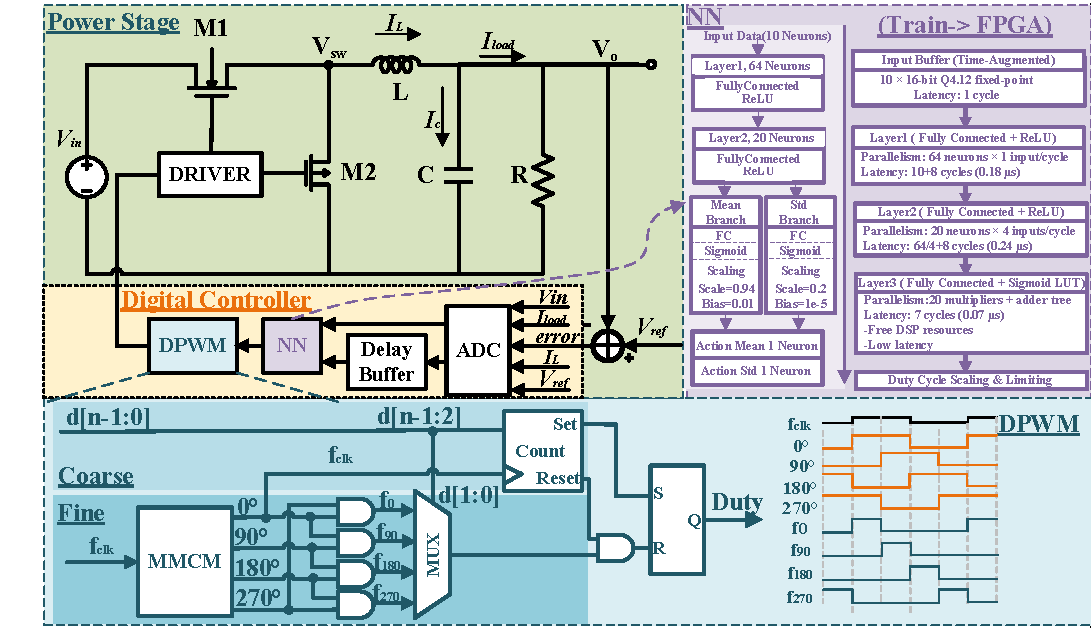
\includegraphics[width=\linewidth]{figures/mea434.pdf}
	\caption{Top-level hardware-algorithm co-design architecture of the DRL-controlled DC-DC converter.}
	\label{fig:top_arch}
\end{figure}

\noindent
where $e_{\text{norm}} = e_t / V_{\text{ref}}$, $k_1 = 1$, and $k_2 = 10$.

To systematically mitigate the sim-to-real gap, the agent is trained offline in a 1 MHz simulation embedded with physical constraints, including soft-start dynamics, precise ADC conversion, and discrete propagation delays. Bounded Gaussian measurement noise ($\pm 15$ mV) alongside wide-range $V_{in}$, $V_{ref}$, and load transients are explicitly injected, but passive component variations are strictly excluded. This deliberate exclusion compels the control policy to extract generalized temporal dynamics instead of overfitting to parameter-specific distributions. Prior to FPGA deployment, the floating-point MLP (10-64-20-1) undergoes Q4.12 fixed-point quantization. Parallelized multipliers and adder trees compress the critical path, achieving 0.50 µs (50 cycles) inference at 100 MHz. A custom 9-bit DPWM ensures synchronous 1 MHz switching. Xilinx Zynq-7020 SoC synthesis utilizes 77\% DSPs, 89\% BRAMs, and 31\% LUTs, a footprint addressable via future ASIC migrations. With a 0.919 W on-chip power consumption, this sub-watt overhead provides a highly viable trade-off between comprehensive dynamic robustness and system efficiency.

\vspace{-10pt}  % 根据需要调整数值（负值减小间距）
\section{Experimental Validation of Multi-Domain Robustness}
\vspace{-5pt}  % 根据需要调整数值（负值减小间距）

The 1 MHz PPO controller is validated on a physical 12 V to 5 V buck prototype. While training convergence over 300 episodes is shown in Fig.~\ref{fig:measure}(a), the policy demonstrates robust zero-shot adaptation to unmodeled physical component drifts. As verified in Fig.~\ref{fig:measure}(b), under $\pm$30\% variations in L (0.47 $\mu$H) and C (44 $\mu$F), output voltage errors strictly remain within [-0.62\%, +0.13\%] and [-0.19\%, -0.01\%]. This validates the intrinsic capability of agent to counteract structural parameter shifts purely by inferring trajectory derivatives from its delay-embedded observation space. Furthermore, simulated dynamic profiles in Fig.~\ref{fig:measure}(c) corroborate consistent regulation across nonlinear CCM/DCM transitions.

The hardware evaluation platform is shown in Fig.~\ref{fig:measure}(d). As shown in Fig.~\ref{fig:measure}(e), the proposed controller maintains steady-state voltage errors below 1\% across input variations (9.5–14.5 V), reference fluctuations (4.5–5.5 V), and full-range load changes (0–1.3 A). The transient oscillograms in Fig.~\ref{fig:measure}(f) corroborate the rapid stabilization capability of agent during severe load transients across the CCM/DCM boundary. The proposed control scheme effectively suppresses the maximum transient voltage deviation to 53 mV, exhibiting rapid dynamic recovery with settling times of 11.5 $\mu$s and 10.5 $\mu$s during step-up (0.1 A to 1 A) and step-down (1 A to 0.1 A) load transitions, respectively.

\begin{figure}[h!]
	\centering
	
\includegraphics[width=\linewidth]{figures/simulation2.pdf}
	\caption{Experimental characterization of PPO-controlled buck converter: (a) Reward curve; (b) Steady-state error vs L/C variations; (c) Simulation results under different operation scenarios; (d) Experimental setup; (e) Steady-state response performance; (f) Dynamic response to load step disturbances.}
	\label{fig:measure}
\end{figure}

\vspace{-25pt}  % 根据需要调整数值（负值减小间距）
\section{Conclusion}
\vspace{-5pt}  % 根据需要调整数值（负值减小间距）

A robust PPO framework integrating delay-embedded states with a sub-watt FPGA inference architecture is proposed for 1 MHz DC-DC converters. Physical validation on a 12 V to 5 V prototype confirms zero-shot policy adaptation to unmodeled L/C parameter drifts, despite their explicit exclusion during training. Furthermore, the controller maintains consistent robustness against CCM/DCM transitions and wide-range $V_{in}/V_{ref}$ fluctuations, achieving $\mu$s-level transient recovery with steady-state errors below 1\%. This co-design paradigm validates robust AI deployment in high-frequency power electronics, optimizing the trade-off between dynamic performance and digital overhead.

\vspace{-10pt}  % 根据需要调整数值（负值减小间距）

\begin{thebibliography}{99}
\small
\setlength{\itemsep}{0pt}
\setlength{\parskip}{0pt}
\bibitem{zhang2026}
J.~Zhang, J.~Xu, Y.~Dai, M.~Yu, X.~Zhang, and H.~Wang, ``Artificial intelligence-based modeling and control strategy for dual active bridge converter with triple phase shift modulation,'' \textit{IEEE Trans. Power Electron.}, vol.~41, no.~1, pp.~494--513, 2026.
\bibitem{ye2024deep}
J.~Ye, H.~Guo, B.~Wang, and X.~Zhang, ``Deep deterministic policy gradient algorithm based reinforcement learning controller for single-inductor multiple-output DC-DC converter,'' \textit{IEEE Trans. Power Electron.}, vol.~39, no.~4, pp.~4078--4090, 2024.
\bibitem{11040024}
C.~Cui, Z.~Fan, T.~Yang, P.~Lin, C.~Gong, and C.~Zhang, ``Domain adaptation-based transfer learning for DRL control implementation of DC microgrids,'' \textit{IEEE Trans. Ind. Electron.}, vol.~72, no.~12, pp.~14344--14355, 2025.


\end{thebibliography}

\end{document}